\documentclass[11pt,twoside]{article}
\usepackage{geometry}
\usepackage{enumerate}
\usepackage{latexsym,booktabs}
\usepackage{amsmath,amssymb}
\usepackage{graphicx}
\usepackage{hyperref}
\usepackage[singlespacing]{setspace}
\usepackage{calc}
\usepackage{listings}
\usepackage{xcolor}
\usepackage{datetime2}
\usepackage[UKenglish]{datetime}

\definecolor{codegrey}{rgb}{0.5, 0.5, 0.5}
\definecolor{darkpurple}{RGB}{151, 10, 232}
\definecolor{backcolour}{rgb}{0.95, 0.95, 0.92}
\definecolor{forestgreen}{RGB}{5, 155, 50}
\definecolor{codeorange}{RGB}{255, 128, 0}

\lstdefinestyle{mystyle}{
    backgroundcolor=\color{backcolour},   
    commentstyle=\color{forestgreen},
    keywordstyle=\color{blue},
    numberstyle=\tiny\color{codegrey},
    identifierstyle=\color{codeorange},
    stringstyle=\color{darkpurple},
    basicstyle=\ttfamily\footnotesize,
    breakatwhitespace=false,         
    breaklines=true,                 
    captionpos=b,                    
    keepspaces=true,                 
    numbers=left,                    
    numbersep=5pt,                  
    showspaces=false,                
    showstringspaces=false,
    showtabs=false,                  
    tabsize=2
}

\lstset{style = mystyle}

\geometry{a4paper,left=2cm,right=2.0cm, top=2cm, bottom=2.0cm}

\newtheorem{Definition}{Definition}
\newtheorem{Theorem}{Theorem}
\newtheorem{Lemma}{Lemma}
\newtheorem{Corollary}{Corollary}
\newtheorem{Proposition}{Proposition}
\newtheorem{Algorithm}{Algorithm}
\numberwithin{Theorem}{section}
\numberwithin{Definition}{section}
\numberwithin{Lemma}{section}
\numberwithin{Algorithm}{section}
\numberwithin{equation}{section}

\newcommand{\dottedline}[1]{\makebox[#1]{.\dotfill}}

\begin{document}

\pagestyle{empty}

% =============================================================================
% Title page
% =============================================================================
\begin{titlepage}
\vspace*{.5em}
\center
\textbf{\Large{The School of Mathematics}} \\
\vspace*{1em}
\begin{figure}[!h]
\centering

\includegraphics[width=180pt]{CentredLogoCMYK.jpg}
\end{figure}
\vspace{2em}
\textbf{\Huge{Estimating Property Types from Street View Images by Applying Neural Network Models}}\\[2em]
\textbf{\LARGE{by}}\\
\vspace{2em}
\textbf{\LARGE{Robin Lin, s2435943}}\\
\vspace{6.5em}
\Large{Dissertation Presented for the Degree of\\
MSc in Statistics with Data Science}\\
\vspace{6.5em}
\Large{June 2023}\\
\vspace{3em}
\Large{Supervised by\\Dr Nicole Augustin and Dr Michael Allerhand}
\vfill
\end{titlepage}

\cleardoublepage

% =============================================================================
% Executive summary, acknowledgments, and own work declaration
% =============================================================================
\begin{center}
\Large{Executive Summary}
\end{center}

Estimating premiums has always been a crucial but tough task for insurance providers, and classifying types of properties is undoubtedly the most essential part. In this project, images from Google street view are provided, and neural network models are constructed to predict property types. Among various models, the simple multi-layer perceptron (MLP) and convolutional neural network (CNN) models are adopted, and it turns out that the CNN model performs better than the MLP model in terms of prediction accuracy, although both models still could not present accurate results. By taking a closer look into the images, crucial observations are found, showing that some of the images are not of good quality, and that different types of properties are usually spotted to have similar shapes. Hence, it is suggested that image data from inside the houses should be provided as supplements to the outdoor street view data.

\clearpage

\begin{center}
\Large{Acknowledgments}
\end{center}

I would like to thank Dr. Nicole Augustin and Dr. Michael Allerhand, the project supervisors, for their careful instructions and patient guidance. I would also like to thank Mr. Gordon Baggott and Ms. Ekaterina Zaytseva, the $2$ staff working in \href{https://www.simplybusiness.co.uk/}{\textit{Simply Business}}, for providing the data, and clarifying details of the project. I am also grateful to Mr. Lennart Hoheisel, the student helper, for his help in my understanding of the ideas of the whole project. Finally, I would like to thank $3$ of my friends, Julia Jose, Will Graham, and Riahn Holcomb, who have provided me with their creative thoughts in solving practical problems.

\clearpage

\begin{center}
\Large{University of Edinburgh – Own Work Declaration}
\end{center}


This sheet must be filled in, signed and dated - your work will not be marked unless this is done.
\vspace{1cm}

Name: \dottedline{8cm}

Matriculation Number: \dottedline{6cm}

Title of work: \dottedline{8cm}

\vspace{1cm}

I confirm that all this work is my own except where indicated, and that I have:
\begin{itemize}
\item	Clearly referenced/listed all sources as appropriate	 				
\item	Referenced and put in inverted commas all quoted text (from books, web, etc)	
\item	Given the sources of all pictures, data etc. that are not my own				
\item	Not made any use of the report(s) or essay(s) of any other student(s) either past 	
or present	
\item	Not sought or used the help of any external professional academic agencies for the work
\item	Acknowledged in appropriate places any help that I have received from others	(e.g. fellow students, technicians, statisticians, external sources)
\item	Complied with any other plagiarism criteria specified in the Course handbook
\end{itemize}

I understand that any false claim for this work will be penalised in accordance with
the University regulations	(\url{https://teaching.maths.ed.ac.uk/main/msc-students/msc-programmes/statistics/data-science/assessment/academic-misconduct}).								

\vspace{1cm}

Signature \dottedline{8cm}

\vspace{5mm}

Date \dottedline{8cm}


\clearpage



% =============================================================================
% Table of contents, tables, and pictures (if applicable)
% =============================================================================
\pagestyle{plain}
\setcounter{page}{1}
\pagenumbering{Roman}

\tableofcontents
\clearpage
\listoftables
\listoffigures
\cleardoublepage

\pagenumbering{arabic}
\setcounter{page}{1}

\nocite{*}
\bibliographystyle{abbrv}
\clearpage

\section{Introduction}
\label{sec:intro}
\subsection{Overview}
\href{https://www.simplybusiness.co.uk/}{\textit{Simply Business}} is one of the largest providers of business and landlord insurance in the UK. Such a provider works on determining premiums that customers need to pay for their property insurance. When the premiums are estimated, various risk factors are taken into account, including the types and sizes of properties, the number of rooms, and the characteristics of the constructions, etc. Among all risk factors, the types of properties are vitally important for insurance companies. A possible reason for that could be the variations in shapes and materials in the construction processes of properties. Such differences could have an impact on whether they are easy to get damaged in various situations. For instance, the ability of a round-shaped facade to avoid being knocked down by strong wind is often higher than that of a flat one. Also, brick houses are not as easily burnt by fire as wood ones. Such information is used by insurance providers to adjust the policies to their customers accordingly.

\subsection{Data Description and Project Objectives}
In this project, the street view images and datasets to be used are provided by \href{https://www.simplybusiness.co.uk/}{\textit{Simply Business}}. Multiple images are extracted from the latest Google street view data, with a unique identity number attached to each of them. Multiple datasets are extracted from \href{https://www.rightmove.co.uk/}{\textit{Rightmove} website}, clearly showing the necessary information of the properties as follows.

\begin{itemize}
    \item Addresses
\item Property Types
\item Numbers of Bedrooms
\item Web Links
\item Location Coordinates
\item Identity Numbers
\end{itemize}






For the images, their property types could be extracted from one of the given datasets by providing the identity numbers attached to them, allowing the types of properties to be linked with the images. The main objectives of this project are to estimate the types of properties by constructing different models given the images from Google street view, and to select a model with the best accuracy, so that the types of properties could be detected automatically. It is worth estimating the types of properties, in that some customers might have failed to reveal the information regarding their properties, or they might have provided the wrong information. Since images from Google street view data are novel, such intuitive and figurative information could be able to reveal the housing status of a customer authentically.

\subsection{Characteristics of the Properties and Street View Images}
As mentioned above, the datasets clearly show the information of the properties. These datasets also share exactly the same attributes, making it easy for us to merge the entries from different datasets into a new data frame. In the new data frame, there are $37,402$ entries in total, and no missing values are found for the property types. However, not every property has an attached street view image. In this case, only the properties with street view images attached would be taken into account in the models. The number of such kind of properties is $35,744$. However, this does not necessarily mean that the number of unique street view images is $35,744$, and in fact a large number of duplicate images are spotted. Although the duplicate images have different identity numbers attached to them, they share exactly the same latitudes and longitudes. In the future models, overfitting issue might occur if a large amount of duplicate images are taken into account in the models, since there would be more noise affecting the performances of the models. In view of this, such duplicate images should be discarded, and there are $15,484$ unique images. In the new data frame, the entries corresponding to the duplicate images should also be removed accordingly. Those entries are the ones with the same values of latitudes and longitudes. The number of unique properties is hence $15,484$.

The unique properties are scattered on the UK map as follows in Figure \ref{fig:locations}. 


\begin{figure}[h]
\centering
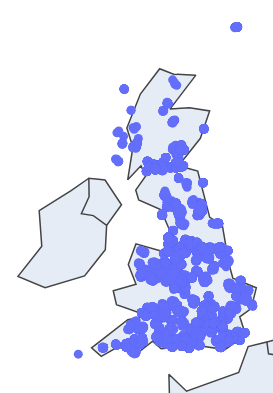
\includegraphics[scale = 1]{1/MSc_LaTeX_SwDS/MSc_LaTeX_SwDS/Plots/Locations.png}
\caption{Locations of the Properties}
\label{fig:locations}
\end{figure}

At first glance, it could be observed that the properties are selected from Great Britain and some other small isles of Britain. By having a closer look into it, it could be observed that the properties are mostly extracted from the middle and south of England, north of Wales, Glasgow, and Edinburgh. There are also a few properties located in the north of England, as well as in the north of Scotland.

There are $4$ types of properties considered in this project, which are detached, flat, semi-detached, and terraced. However, there are $5$ classes in the variable “property types”, and the other class not specified above is the “unknown” one. When street view images are labelled as “unknown”, there could be at least one possible type of property, or it could be the case where none of the $4$ types best describe the characteristics of the properties in the street view images. The percentages of the $5$ classes are shown as follows in Figure \ref{fig:pie}. 

\begin{figure}[h]
\centering
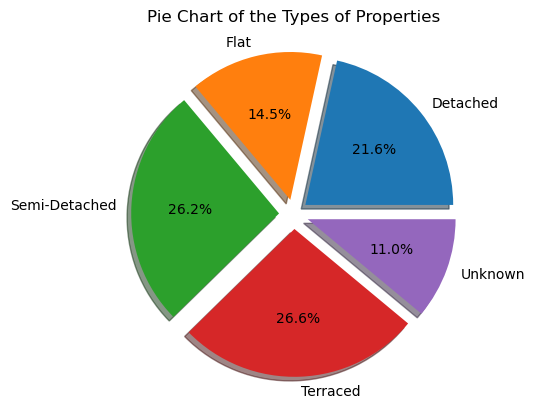
\includegraphics[scale = .7]{1/MSc_LaTeX_SwDS/MSc_LaTeX_SwDS/Plots/Pie.png}
\caption{Pie Chart of the Types of Properties}
\label{fig:pie}
\end{figure}

From the pie chart, it could be observed that the classes are not evenly divided, indicating that the data set is imbalanced. An imbalanced dataset could be harmful in the models. When a model is being trained, it could probably keep predicting the classes that have higher proportions, in order that a higher accuracy in the training sets could be achieved. However, when it comes to validating and testing the model, the performances of classes with lower proportions might not be decent enough. This is because classes with lower proportions might not be able to learn as much as the other classes do, leading to lower accuracy in model prediction. In view of this, some perturbations are to be made in the loss function, which would be discussed in later sections.

As mentioned above, there are $5$ classes in the variable “property types”, and one of the classes is “unknown”. It is crucial to discuss whether to have the images labelled as “unknown” kept as they are, or to have them discarded, as this might have an impact on the performances of the models. There is no harm in looking at some example images first. As mentioned above, it could be the case where none of the 4 types best describe the characteristics of the properties. As shown in Figure \ref{fig:unknown_green_road}, if images mostly contain objects that are in green, such as trees or forests, or when they contain a road without a house, the models might learn them as a pattern, and classify property types correctly as “unknown”. However, such a case only occurs in a very small portion of images. 

\begin{figure}[h]
\centering
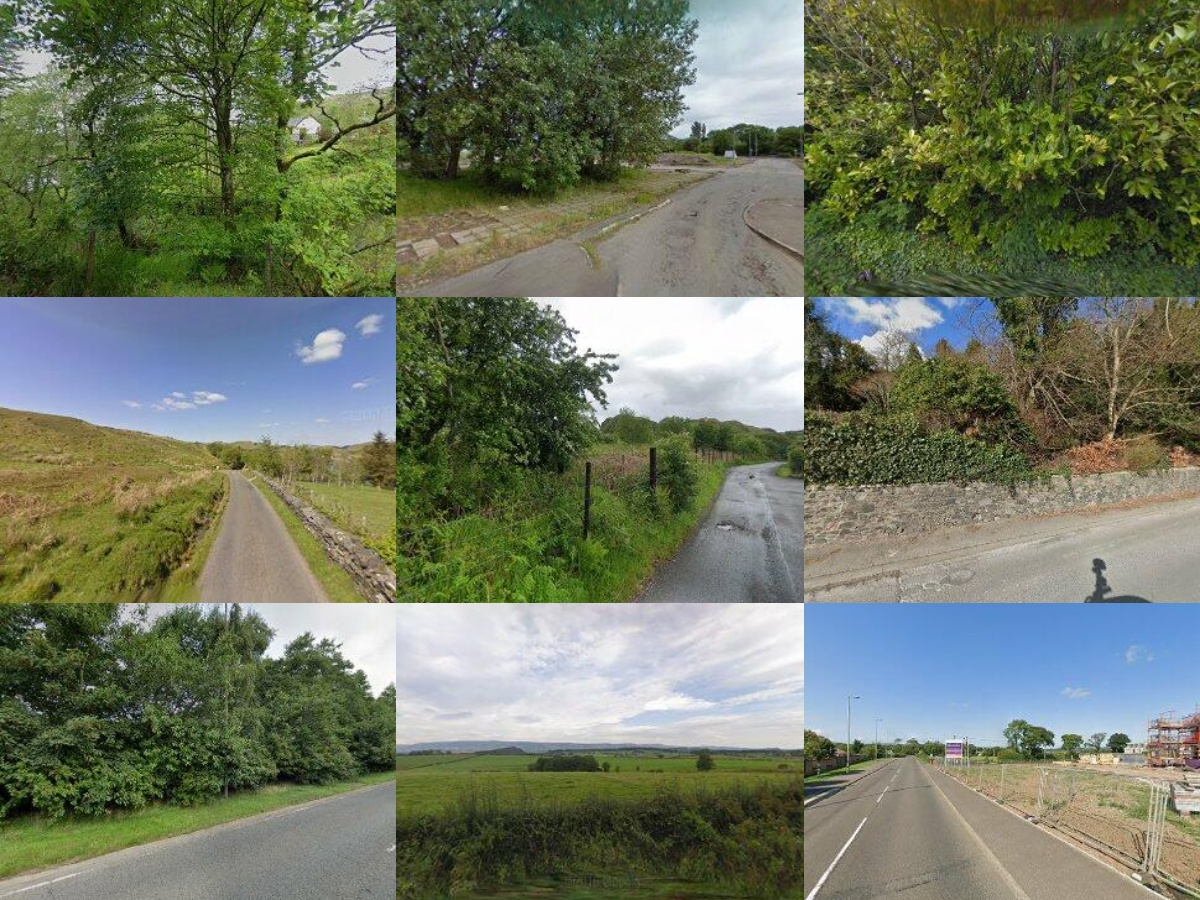
\includegraphics[scale = .2]{1/MSc_LaTeX_SwDS/MSc_LaTeX_SwDS/Labelled Unknown/no_houses.jpg}
\caption{Examples of Properties Labelled “Unknown” without a House}
\label{fig:unknown_green_road}
\end{figure}

In general, there are houses in most images labelled “unknown”, so there is a greater chance that at least one possible type of property is in the images, as shown in Figure \ref{fig:unknown_houses}. 

\begin{figure}[h]
\centering
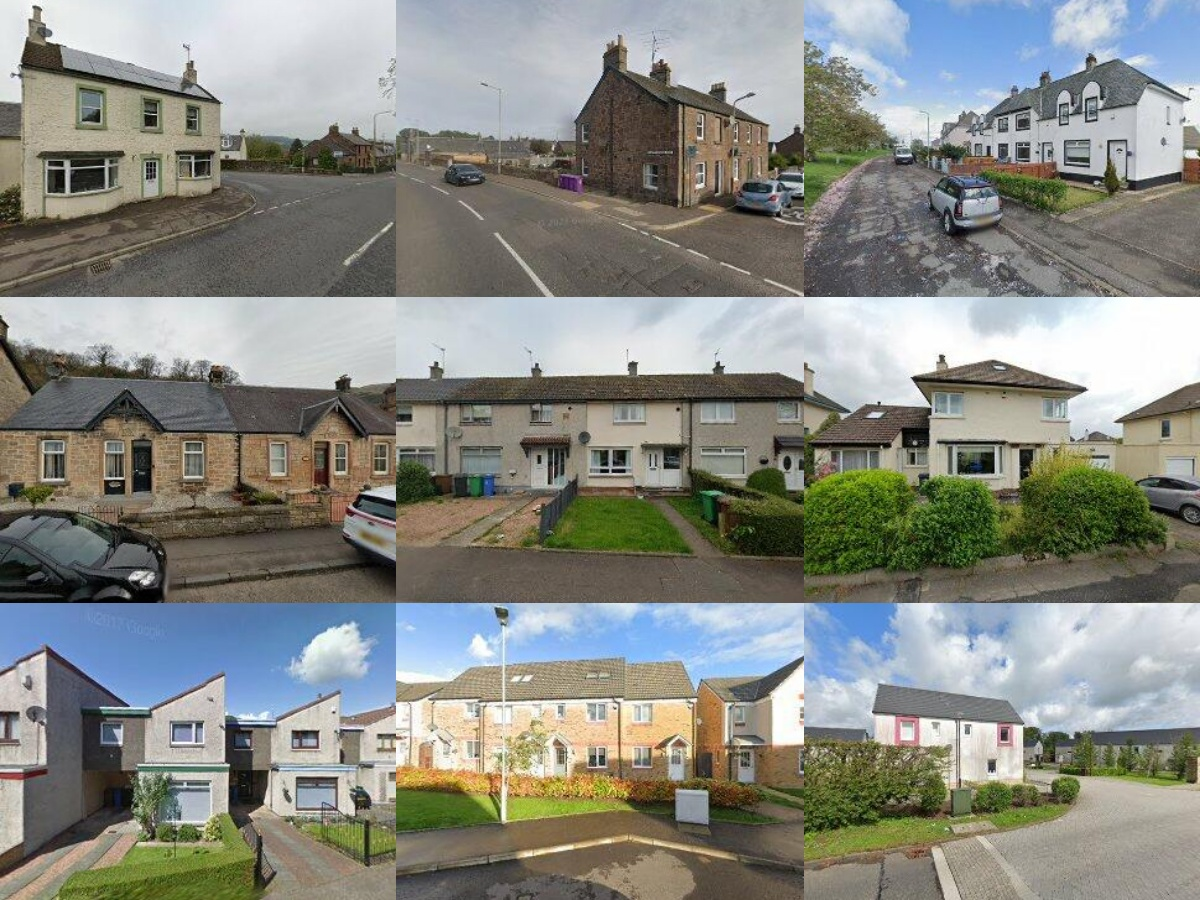
\includegraphics[scale = .2]{1/MSc_LaTeX_SwDS/MSc_LaTeX_SwDS/Labelled Unknown/apparent_houses.jpg}
\caption{Examples of Properties Labelled “Unknown” with Houses}
\label{fig:unknown_houses}
\end{figure}

When models are being trained, the contours of the houses might be captured and sketched by them. After the models are trained, they should be validated and tested, and the contours are key information in classifying the types of houses. This could lead to a situation where the models classify objects in the images as one of the $4$ types of properties, instead of classifying them as “unknown”, indicating that the accuracy of validation and testing would be very low. Moreover, “unknown” is not a type of property being widely acknowledged by people, and hence it does not make any sense to classify the images as this type. Therefore, the images labelled “unknown” are ignored, along with their corresponding entries in the new data frame. The number of images to be considered should hence be $13,775$.

\subsection{A Literature Review on Image Classification Models}
A brief review of the literature is provided, presenting the models applied in classification of images, especially Google street view images, in recent years. In 2016, the authors of \cite{ahmed2016house} extracted visual and textural features, and fed them into a multi-layer perceptron (MLP) model and a support vector regression (SVR) model. They concluded that their MLP model performed better than their SVR model. In 2017, the authors of \cite{law2017application} applied the convolutional neural network (CNN) model to classify the frontages of street view images in Greater London and found decent results in their model. In 2018, the authors of \cite{kang2018building} applied VGG16, a special kind of CNN model, to classify the facade structures from Google street view images, and achieved high accuracy. In 2019, the authors of \cite{law2019take} applied CNN and Generalised Additive Model (GAM) to the Google street view images from different angles in predicting house prices in London, and found promising results. In 2020, the authors of \cite{avelar2020superpixel} adopted Graph Neural Network (GNN) models in classifying superpixel images, which was an unprecedented experiment, and they successfully classified panoramas. Finally, in 2021, the authors of \cite{maniat2021deep} also adopted VGG16 to detect visual cracks in pavement images extracted from Google street view, and managed to classify those images into different categories of cracks.

From the above literature, it could be observed that people tend to use CNN, especially the newly invented VGG16, to classify street view images. There are cases where people use the traditional MLP and SVR models. In this project, more than $10,000$ images are to be trained, and it does not seem time-efficient to train such a large amount of images using SVR models. Moreover, VGG16 model looks too fancy to be implemented, since such kind of model has a complex structure, and overfitting issue might occur more easily when such a model is adopted. Therefore, simple MLP and CNN models are adopted in this paper.

\section{Preliminary Settings}
\label{sec:prelim}
\subsection{Downsizing Images}
The street view images are reformatted into matrices with $3$ axes. The first axis describes the height of an image, and there are $320$ pixels along this axis. The second one describes the width of an image, and there are also $320$ pixels along this axis. The third one describes the number of primary colours, and there are $3$. After reformatting, $307, 200$ pixel values are generated for each image, and such values are integers ranging from $0$ to $255$. However, there could be an issue of memory if a large amount of features are taken into account in constructing models. A possible way to avoid it could be applying dimensionality reduction techniques, including principle component analysis (PCA), and factor analysis. However, chances are that crucial information might be lost when applying such techniques. For instance, contours of the houses might be necessary for image classification, and if some of those key pixels are missing, models might provide ridiculous results, such as classifying a flat as a terraced one. In view of this, dimensionality reduction techniques would not be the best option. Another possible way could be extracting features by applying algorithms like autoencoder, or diffusion map, etc. However, none of these algorithms seem time-efficient in dealing with such a large scale of features in the images. The fastest, and perhaps the most straightforward method is resizing those images to a lower resolution. This is about merging, and averaging neighbouring pixels, and it preserves the key information in the images, since downsizing them would preserve the information of the contours of houses, which might be crucial in modelling. In this project, the heights and widths of the images are downsized to $64$ pixels. The main advantage of doing so is that training a model would not be extremely time consuming.

\subsection{Normalising Pixel Values}
As mentioned above, the pixel values range from $0$ to $255$. The first thing that we should think about is to normalise these values, so that they range from $0$ to $1$. There are some good reasons for this regarding how the models update the weights. For neural network models, the weights in a certain iteration are updated by adding the product of the learning rate and the gradient to the weights in the previous iteration. If the pixel values were not scaled, the corrections that they might have produced would vary from one another. In other words, some weights might be over-corrected, while some others might be under-corrected. In order to make similar corrections to the weights, such pixel values should be normalised. Typically, in this case, the normalisation process could simply be done by dividing the pixel values by $255$.

\subsection{One Hot Encoding}
For types of properties, the categorical outcome variable, one hot encoding is applied to convert it into the form of numerical values. Such an encoding method preserves norminality of the variable, and ensures that the models could keep learning patterns.

\subsection{Train-Validation-Test Split}
The models adopted in this paper are neural network models. In order to avoid overfitting, it is necessary to split the dataset into different groups. In this project, the dataset is split into non-overlapping training, validation, and testing sets by randomly selecting an integer-valued seed. Among the $3$ sets, there are $70\%$ of the data in the training set, $20\%$ in the validation set, and $10\%$ in the testing set.

\section{Modelling}

\subsection{Models}
As mentioned above, the MLP and CNN models are the $2$ models that we have chosen. Some basic descriptions are provided as follows.

\subsubsection{MLP Model}
The basic structure of our MLP model is shown in Figure \ref{fig:mlp}.

\begin{figure}[h]
\centering
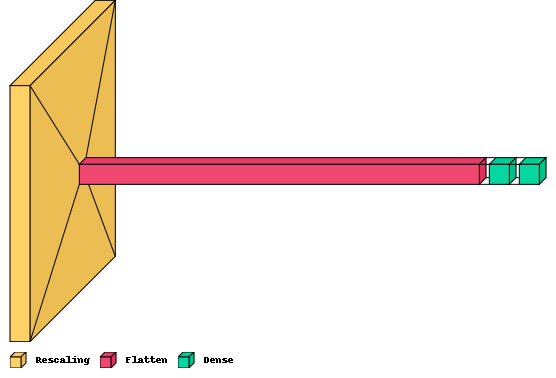
\includegraphics[width = .6\textwidth]{1/MSc_LaTeX_SwDS/MSc_LaTeX_SwDS/Plots/mlpvisual.png}
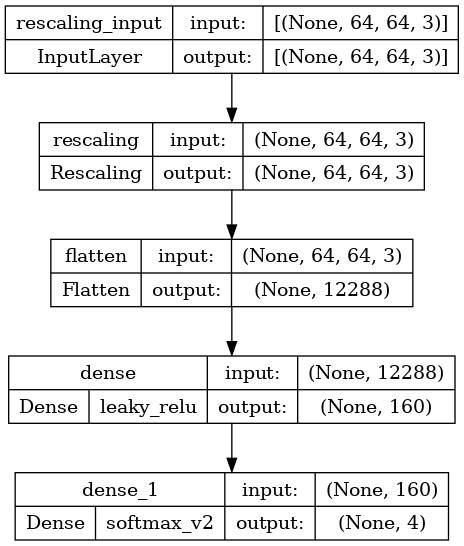
\includegraphics[scale = .4]{1/MSc_LaTeX_SwDS/MSc_LaTeX_SwDS/Plots/mlp.png}
\caption{Structure of MLP}
\label{fig:mlp}
\end{figure}

As shown above, the images are normalised, and flattened, so that the pixel values range from $0$ to $1$, and they are reformatted into vectors. There is only $1$ hidden layer in this model, with $160$ neurons, and the output layer has $4$ neurons, outputting $4$ different types of properties.

\subsubsection{CNN Model}
The basic structure of our CNN model is shown in Figure \ref{fig:cnn}.

\begin{figure}[h]
\centering
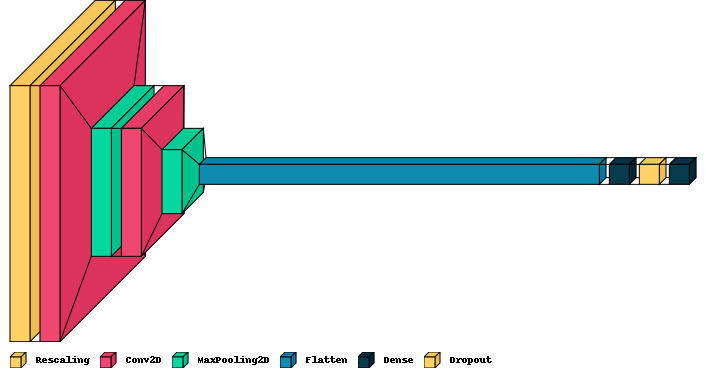
\includegraphics[width = .7\textwidth]{1/MSc_LaTeX_SwDS/MSc_LaTeX_SwDS/Plots/cnnvisual.png}
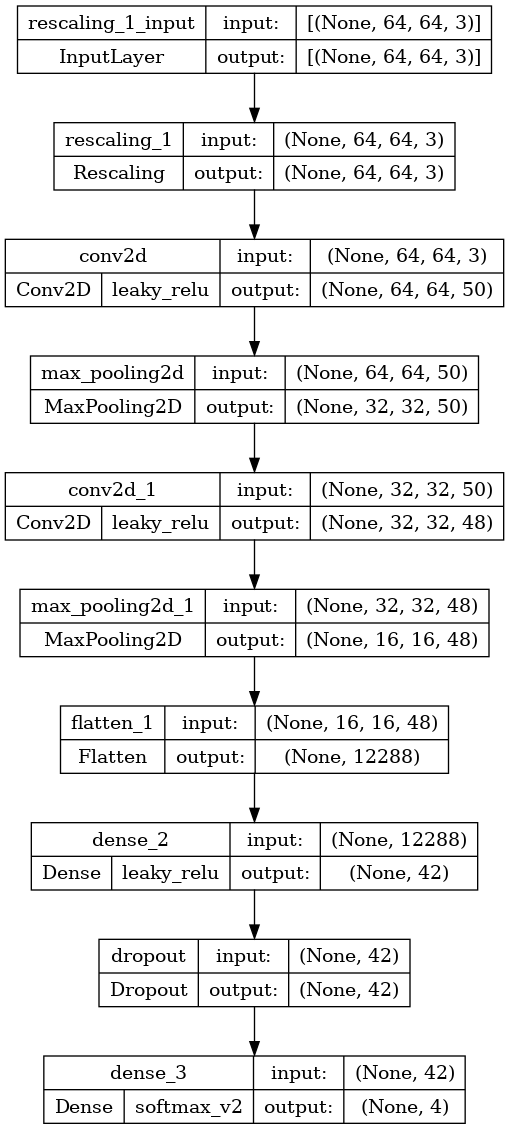
\includegraphics[width = .3\textwidth]{1/MSc_LaTeX_SwDS/MSc_LaTeX_SwDS/Plots/cnn.png}
\caption{Structure of CNN}
\label{fig:cnn}
\end{figure}

As shown above, the images are normalised first. They are then passed in through a $2$-dimensional convolutional layer, outputting a space with $50$ dimensions, and the convolution window has height and width of 4 pixels. The size of output is the same as that of input. Following this, the results are passed in through a $2$-dimensional pooling layer in order to reduce the size of a matrix, and the maximum value would be extracted over a $2$ pixels by $2$ pixels pooling window. After that, the other convolutional and pooling layers are constructed similarly as before, but this time the output space of the convolutional layer has $48$ dimensions. In the next step, the results are passed in through a flatten layer, a fully connected layer with $42$ neurons, a dropout layer with dropout rate of a quarter, and an output layer outputting $4$ types of properties.

\subsection{Selecting Activation Functions}
\subsubsection{ReLU or Leaky ReLU?}
ReLU stands for rectified linear unit. Such an activation function returns exactly the input when it is non-negative, and returns $0$ when it is negative. Compared with sigmoid and hyperbolic tangent activation functions, it does not suffer from the problem of vanishing gradient. When one of sigmoid and hyperbolic tangent activation functions is applied, the gradient has an upper bound, and the further the inputs are from $0$, the smaller the gradient would be. This indicates that the models learn the patterns more slowly when there are multiple layers, and hence the weights would barely update. In order that the models could be persistently learn patterns in the images, ReLU is a better choice compared to sigmoid and hyperbolic tangent activation functions.

Leaky ReLU stands for leaky rectified linear unit. It returns exactly the same value as it is in ReLU when the input is non-negative, but for negative inputs, it has a small slope. Such a small slope is almost invisible, but it is super powerful that it achieves what a ReLU function would not be able to accomplish. When the inputs are negative, ReLU function keeps outputting $0$ all the time, making the neurons inactive. In this case, models would no longer learn anything. However, the leaky ReLU function outputs a non-zero value when the inputs are negative, triggering the neurons to learn the patterns, so that the weights could be updated. This is useful, since the street view images might contain noise, and adopting such an activation function would make models more robust. 

By and large, the leaky ReLU activation function is applied in all of the layers that need an activation function, except for the output layers of the models.

\subsubsection{Why Softmax in the Output Layer?}
In this project, there are $4$ types of properties, as mentioned above. This is a multi-class classification problem, so the activation functions for binary class classification are inappropriate in the output layer. In this case, a typical activation function placed in the output layer is the \textit{softmax} function. In short, \textit{softmax} function converts the inputs into different probabilities that sum up to $1$. In neural network models, these probabilities refer to the likelihoods of predicting different classes.

\subsection{Choosing an Optimisation Algorithm}
The optimisation algorithm we have chosen for the models is Adam. This is by far the best optimisation algorithm in constructing neural network models, and it has several advantages. Firstly, it does not require a large amount of memory, and it is simple and effective in its implementation. It is also capable of problems having a large amount of data, especially for such a massive image classification problem containing $13,775$ street view images. Finally, the hyper-parameters are rather easy to tune and interpret, making it easy to design Adam for different deep learning problems.

\subsection{Choosing a Batch Size}
In neural network models, the batch size refers to the number of samples used to update the weights. The larger the batch size, the smaller the number of iterations in an epoch. In practical experiments, the larger the batch size, the shorter the training time in an epoch, and the larger the variation in the validation accuracy. The smaller the batch size, the longer the training time in an epoch, and the higher the risk of encountering the issue of overfitting. In order to achieve a high and robust validation accuracy, a trade-off between them should be taken into account. In the models, the batch size is selected to be $50$, ensuring that the training time is not that long, and the validation accuracy grows steadily. 

\subsection{Monitoring the Models}
\subsubsection{Epochs}
In neural network models, an epoch refers to a complete training process for all data in the training set. The more the epochs are, the more the chances for the models to learn the patterns in the training set. However, it is also possible that the overfitting issue might occur. In order that this issue could be avoided, the models should be terminated from training when the validation accuracy is not getting any higher for several epochs. In this project, the models terminate from training if the validation accuracy is not improving after $5$ epochs in a row. This saves the training time considerably, and prevents the models from learning too much noise.

\subsubsection{Learning Rates}
The default learning rate of the Adam algorithm is $10^{-3}$. However, in the models, the learning rate should not be a constant, since there is neither assumptions that the problem is a convex one, nor assertions that the validation accuracy is bound to converge. In our case, the learning rates should be adjusted accordingly based on the performances on the validation accuracy in each epoch. The initial value of the learning rate is set to be half of the default value, $i.e.$, $5 \times 10^{-4}$, since we do not wish the models to learn greedily at the very beginning, avoiding that the possible low validation accuracy might be encountered. Every time the accuracy decreases, or when it fails to reach the highest value in previous epochs, the learning rate is multiplied by $4 \times 10 ^ {-2}$. Usually, the models would learn the patterns effectively when the learning rate ranges from around $10^{-6}$ to around $10^{-3}$ within the first $7$ or $8$ epochs, and after that, the validation accuracy starts to converge.

\subsection{Assigning Class Weights to the Loss Function}
The loss function we are using in the models is the categorical cross entropy loss. According to \cite{chollet2021deep}, the categorical cross entropy loss measures the discrepancy between the distributions of the true outcomes and the predicted ones. When such a loss function is minimised, the models are trained in a way that the predictions gradually approach as closely as possible to the true outcomes. 

As mentioned above, the dataset is an imbalanced one, and hence the loss function is to be adjusted. The adjustment that we have made is to assign weights to the $4$ classes, and the more the data in a class, the less the weight they would be assigned, vice versa. The reason of doing so is rather simple. By assigning a lower weight to a class having more data, the models take into account the classes having less data, and avoids being biased towards the classes having more data when predicting outcomes of the validation and testing sets. In order to compute the weight for each class, the total number of samples in the training set, total number of classes, and the number of samples in each class of the training set are required. For each class, the product of the number of classes and the number of samples in this class is calculated at first. The weight for this class is represented by the ratio between the total number of samples and the product mentioned above. After the weights are calculated, they are taken into account in calculating the loss, enabling the models to learn more patterns from the classes having less samples.

\subsection{Regularisation}

\subsubsection{$L_1$ or $L_2$?}
$L_1$-regularisation adds to the loss function the sum of absolute values of hyper-parameters in the models multiplied by a regularisation parameter, and $L_2$-regularisation adds to the loss function the sum of squares of hyper-parameters in the models multiplied by a regularisation parameter. In this project, $L_1$-regularisation technique is applied to the output layers of the $2$ models, since we would like to penalise the hyper-parameters strictly, so that a sparse model could be promoted, making more hyper-parameters shrink exactly towards $0$. In this way, the noise that the models could learn would be limited.

\subsubsection{Regularisers}
There are different kinds of regularisers to be tuned in the output layers of the models. The bias regulariser penalises the bias, the kernel regulariser penalises the hyper-parameters except for the bias, and the activity regulariser penalises the output. According to our experiments, the models have relatively high validation and testing performances if the regularisation parameter for the kernel regulariser is set to be $10^{-5}$, and the ones for the bias and activity regularisers are set to be $10$.

\subsubsection{Dropout Layer in CNN}
In order to avoid overfitting, a dropout layer is introduced in between the fully-connected layer and the output layer in the CNN model. Such a layer aims at making part of the neurons inactive, allowing for later batches in the training set to learn the patterns as much as possible. In our CNN model, a quarter of the neurons are dropped out in the fully connected layer.

\section{Results and Discussions}
\label{sec:results}

\subsection{Results of the $2$ models}
There might be different ways of splitting a dataset when different seeds are set up, and hence the results might be slightly different. Normally, for MLP models, we could get an accuracy from roughly $40\%$ to $44\%$ for the testing data, and for CNN models, such an accuracy ranges roughly from $43\%$ to $47\%$.

\subsubsection{MLP Model}

Figure \ref{fig:mlpacc} shows the changes in accuracy and loss in each epoch.

\begin{figure}[h]
\centering
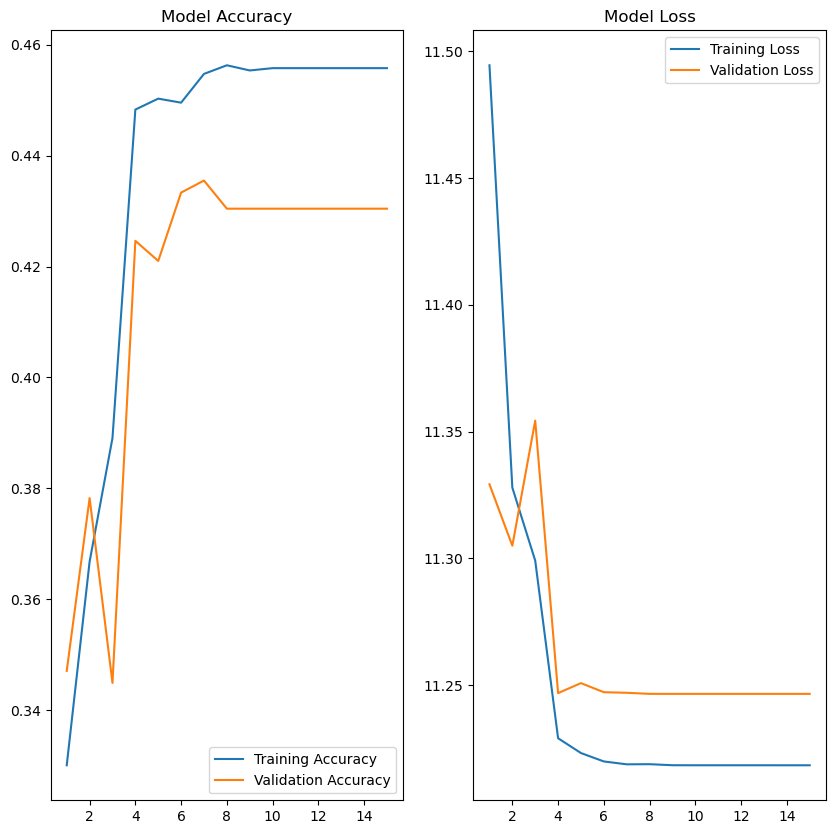
\includegraphics[scale = .55]{1/MSc_LaTeX_SwDS/MSc_LaTeX_SwDS/Plots/mlpacc.png}
\caption{Changes in Accuracy and Loss of the MLP Model}
\label{fig:mlpacc}
\end{figure}

Figure \ref{fig:mlpconf} shows the confusion matrix of the property types in the testing set.

\begin{figure}[h]
\centering
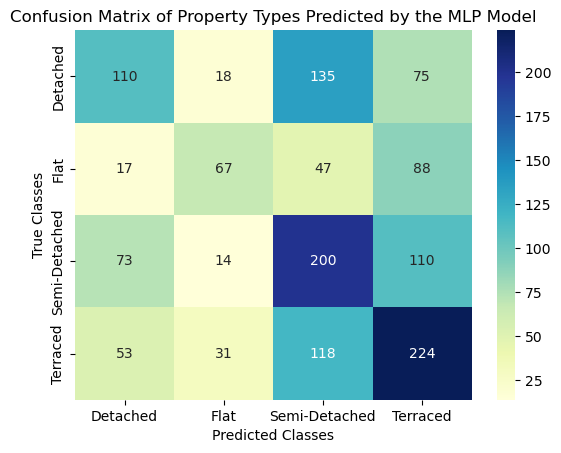
\includegraphics[scale = 1]{1/MSc_LaTeX_SwDS/MSc_LaTeX_SwDS/Plots/mlpconfmat.png}
\caption{Confusion Matrix of the Testing Set in the MLP Model}
\label{fig:mlpconf}
\end{figure}

Table \ref{tab:mlp} reports the classification results in the testing set.

\begin{table}[h]
\centering

\scalebox{1.5}{
\begin{tabular}{c|cc|c|c|}
\cline{2-5}
                                    & \multicolumn{1}{c|}{Precision} & Recall & $F_1$-score & Support \\ \hline
\multicolumn{1}{|c|}{Detached}      & \multicolumn{1}{c|}{0.43}      & 0.33   & 0.37     & 338     \\ \hline
\multicolumn{1}{|c|}{Flat}          & \multicolumn{1}{c|}{0.52}      & 0.31   & 0.38     & 219     \\ \hline
\multicolumn{1}{|c|}{Semi-Detached} & \multicolumn{1}{c|}{0.40}      & 0.50   & 0.45     & 397     \\ \hline
\multicolumn{1}{|c|}{Terraced}      & \multicolumn{1}{c|}{0.45}      & 0.53   & 0.49     & 426     \\ \hline
\multicolumn{1}{|c|}{Accuracy}      &                                &        & 0.44     & 1380    \\ \hline
\multicolumn{1}{|c|}{Macro Avg}     & \multicolumn{1}{c|}{0.45}      & 0.42   & 0.42     & 1380    \\ \hline
\multicolumn{1}{|c|}{Weighted Avg}  & \multicolumn{1}{c|}{0.44}      & 0.44   & 0.43     & 1380    \\ \hline
\end{tabular}
}

\caption{Classification Report of the MLP Model}
\label{tab:mlp}

\end{table}
From the results obtained, the MLP model is not that accurate enough. We could see that there are less samples in classes of  “detached” and  “flat”, and among these properties, only a small portion is predicted by the model. Compared with the other portions, these portions are way smaller, indicating that the model tends to predict the classes having more samples. 

\subsubsection{CNN Model}

Figure \ref{fig:cnnacc} shows the changes in accuracy and loss in each epoch.

\begin{figure}[h]
\centering
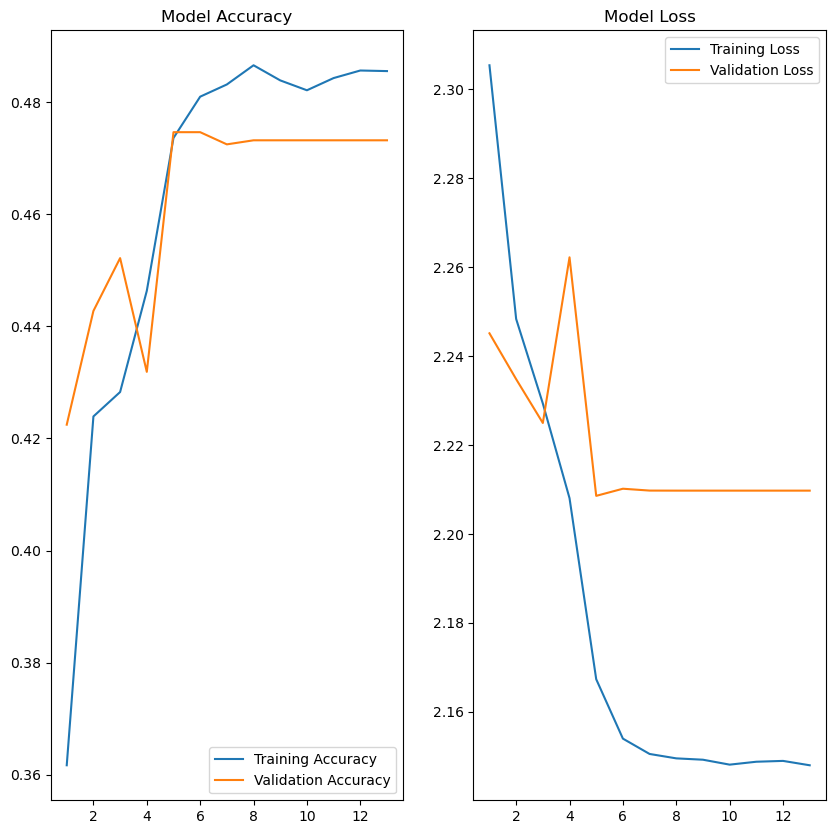
\includegraphics[scale = .4]{1/MSc_LaTeX_SwDS/MSc_LaTeX_SwDS/Plots/cnn2acc.png}
\caption{Changes in Accuracy and Loss of the CNN Model}
\label{fig:cnnacc}
\end{figure}

\newpage

Figure \ref{fig:cnnconf} shows  the confusion matrix of the property types in the testing set.

\begin{figure}[h]
\centering
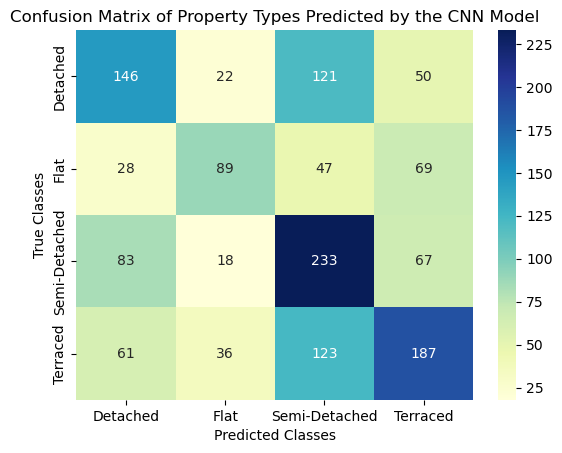
\includegraphics[scale = .79]{1/MSc_LaTeX_SwDS/MSc_LaTeX_SwDS/Plots/cnn2confmat.png}
\caption{Confusion Matrix of the Testing Set in the CNN Model}
\label{fig:cnnconf}
\end{figure}

\newpage
Table \ref{tab:cnn} reports the classification results in the testing set.

\begin{table}[h]
\centering
\scalebox{1.5}{
\begin{tabular}{c|cc|c|c|}
\cline{2-5}
                                    & \multicolumn{1}{c|}{Precision} & Recall & $F_1$-score & Support \\ \hline
\multicolumn{1}{|c|}{Detached}      & \multicolumn{1}{c|}{0.47}      & 0.47   & 0.47     & 339     \\ \hline
\multicolumn{1}{|c|}{Flat}          & \multicolumn{1}{c|}{0.53}      & 0.40   & 0.45     & 233     \\ \hline
\multicolumn{1}{|c|}{Semi-Detached} & \multicolumn{1}{c|}{0.44}      & 0.57   & 0.50     & 401     \\ \hline
\multicolumn{1}{|c|}{Terraced}      & \multicolumn{1}{c|}{0.48}      & 0.42   & 0.45     & 407     \\ \hline
\multicolumn{1}{|c|}{Accuracy}      &                                &        & 0.47     & 1380    \\ \hline
\multicolumn{1}{|c|}{Macro Avg}     & \multicolumn{1}{c|}{0.48}      & 0.46   & 0.47     & 1380    \\ \hline
\multicolumn{1}{|c|}{Weighted Avg}  & \multicolumn{1}{c|}{0.48}      & 0.47   & 0.47     & 1380    \\ \hline
\end{tabular}
}

\caption{Classification Report of the CNN Model}
\label{tab:cnn}

\end{table}



From the results obtained, the CNN model is also not that accurate enough, but the overall accuracy is higher than that of the MLP model. Surprisingly, we observe that for samples in classes of  “detached” and  “flat”, more predictions are correctly made by the model, indicating that the model takes into account the classes having less samples. We could also observe that the $F_1$-scores are similar in each class, indicating that the predictions do not depend much on the numbers of data in different classes. Hence, the CNN model is selected as the best one.

\subsection{Error Analysis}
From the confusion matrix shown in Figure \ref{fig:cnnconf}, there are a bunch of houses labelled “detached” and “terraced” being wrongly classified as “semi-detached”, which catches our eyes. Generally speaking, detached houses are standalone ones, semi-detached ones are $2$ properties sharing a wall in between, and terraced ones are multiple properties sharing walls with their neighbours. By taking a closer look into the images, it could be observed that some longer detached houses or shorter terraced houses look somehow similarly to semi-detached ones in their shapes, which explains why there are a lot of detached and terraced houses being classified as semi-detached ones. 

In addition, a large amount of images are not captured in a perfect angle, and some images are blurry, or obstructed by some trees, which would also worsen the performance of the model. A better solution to the issues would be taking into account the images from inside the houses, and not relying only on the street view data. By doing so, structures inside the houses would be clear. For instance, we might not be able to distinguish whether some houses share common walls, or a corridor from the street view data, but if pictures from inside the houses are provided, everything would be clear.

\section{Conclusions}
In this work, the MLP and CNN models are proposed in classifying types of properties using Google street view images, and CNN performs better in terms of the accuracy of the testing set. However, the accuracy of CNN in the testing set is not decent enough, showing that there might be issues within the images. By taking a closer look into the images, it could be observed that different types of properties might share similar structures that the model could not distinguish. It could also be observed that a large amount of images are somehow blurry, and some houses are crooked, making it challenging for the models to learn. Providing more image data from inside the houses are suggested, and the novel method suggested in \cite{avelar2020superpixel} might also help classifying types of properties.
\newpage

%the entries have to be in the file literature.bib
\bibliography{literature}


\end{document}
